\documentclass[a4paper]{article}
\usepackage[margin=1in]{geometry}
\usepackage{graphicx}
\usepackage{hyperref}
\usepackage{amsmath}
\usepackage{booktabs}
\usepackage{subcaption}
\usepackage{tikz}
\usepackage{pgfplots}

\title{\textbf{VE216 Lab 1 Report\\LTI Systems}}
\author{
    \Large Han Yibei
    \normalsize 519370910123
}
\date{\today}

\begin{document}
    \maketitle
    \tableofcontents
    \newpage




    \section{Objectives}
    \begin{itemize}
        \item Measure the output response of the series RC circuit for a variety of inputs, including a step, a
        combination of a step and a ramp, and a sinusoid
        \item svCompare results to those computed as part of pre-lab assignment
    \end{itemize}






    \section{Theoretical Background}
    \subsection{Linear Circuit as a linear system}
    An RC circuit can be expressed by following equation:
    \begin{equation}
        RC\frac{dV_{out}(t)}{dt} + V_{out}(t) = V_{in}(t)    
    \end{equation}
    We can calculate $V_{out}$ through solving this equation:
    \begin{equation}
        V_{out}(t) = V_0e^{-t/RC} + \int_0^t \frac{1}{RC}e^{-(t-\tau)/RC}V_{in}(\tau)d\tau
    \end{equation}
   So an RC circuit is an LTI system if and only if $V_{out}=V_0=0$. 

    \subsection{Impulse Response}
    The impulse response, $h(t)$, is the output response when the input of the system is a delta function, $\delta(t)$. And in the experiment, the delta function is simulated by two step function with short interval, $p_\Delta(t) = \frac{1}{\Delta}(u(t)-u(t-\Delta))$ for $\Delta > 0$ and $\Delta \rightarrow 0$.

    \subsection{Step Response}
    The impulse response can be computed from the unit step response by calculating the derivative of the step response as followed. 
    \begin{equation}
        \frac{dy(t)}{dt} = \frac{dx(t)}{dt}*h(t)
    \end{equation}

    \section{Experiment Procedures}
    \paragraph{Step Response}
    Set the function generator with: square wave, Vpp 1V, frequency 100Hz; oscillator with: CH1 200mV/div, CH2 200mv/div, Time: 2ms.
    \paragraph{Pulse Response}
    Set the function generator with: frequency 100hz; For the first trial: width 1ms, A 100mV; For the second trial: width 0.5ms, A 200mV;
    \paragraph{Ramp Response}
    Set the function generator with: ramp, Vpp 100mV, frequency 100Hz;
    \paragraph{Sine Response}
    Set the function generator with: Vpp 10V, frequency 50, 500, 5kHz respectively;



    \section{Experimental Results}
    \subsection{Step Response}
    The experimental step response is shown in \autoref{step}. For the theoretical output, we can calculate the solution of \text{Eq.1} when $V_{in}(t) = u(t)$: 
    \begin{equation}
        V_{out} = (1 - e^{-1000t})u(t)
    \end{equation}
    And the plot is shown in \autoref{steptrue} Also, we can see the comparison between the experimental and theoratical result.

    We can see that the experimental result is similar to the theoretical result.
   \begin{figure}[h]
        \centering
        \begin{subfigure}{0.4\textwidth}
            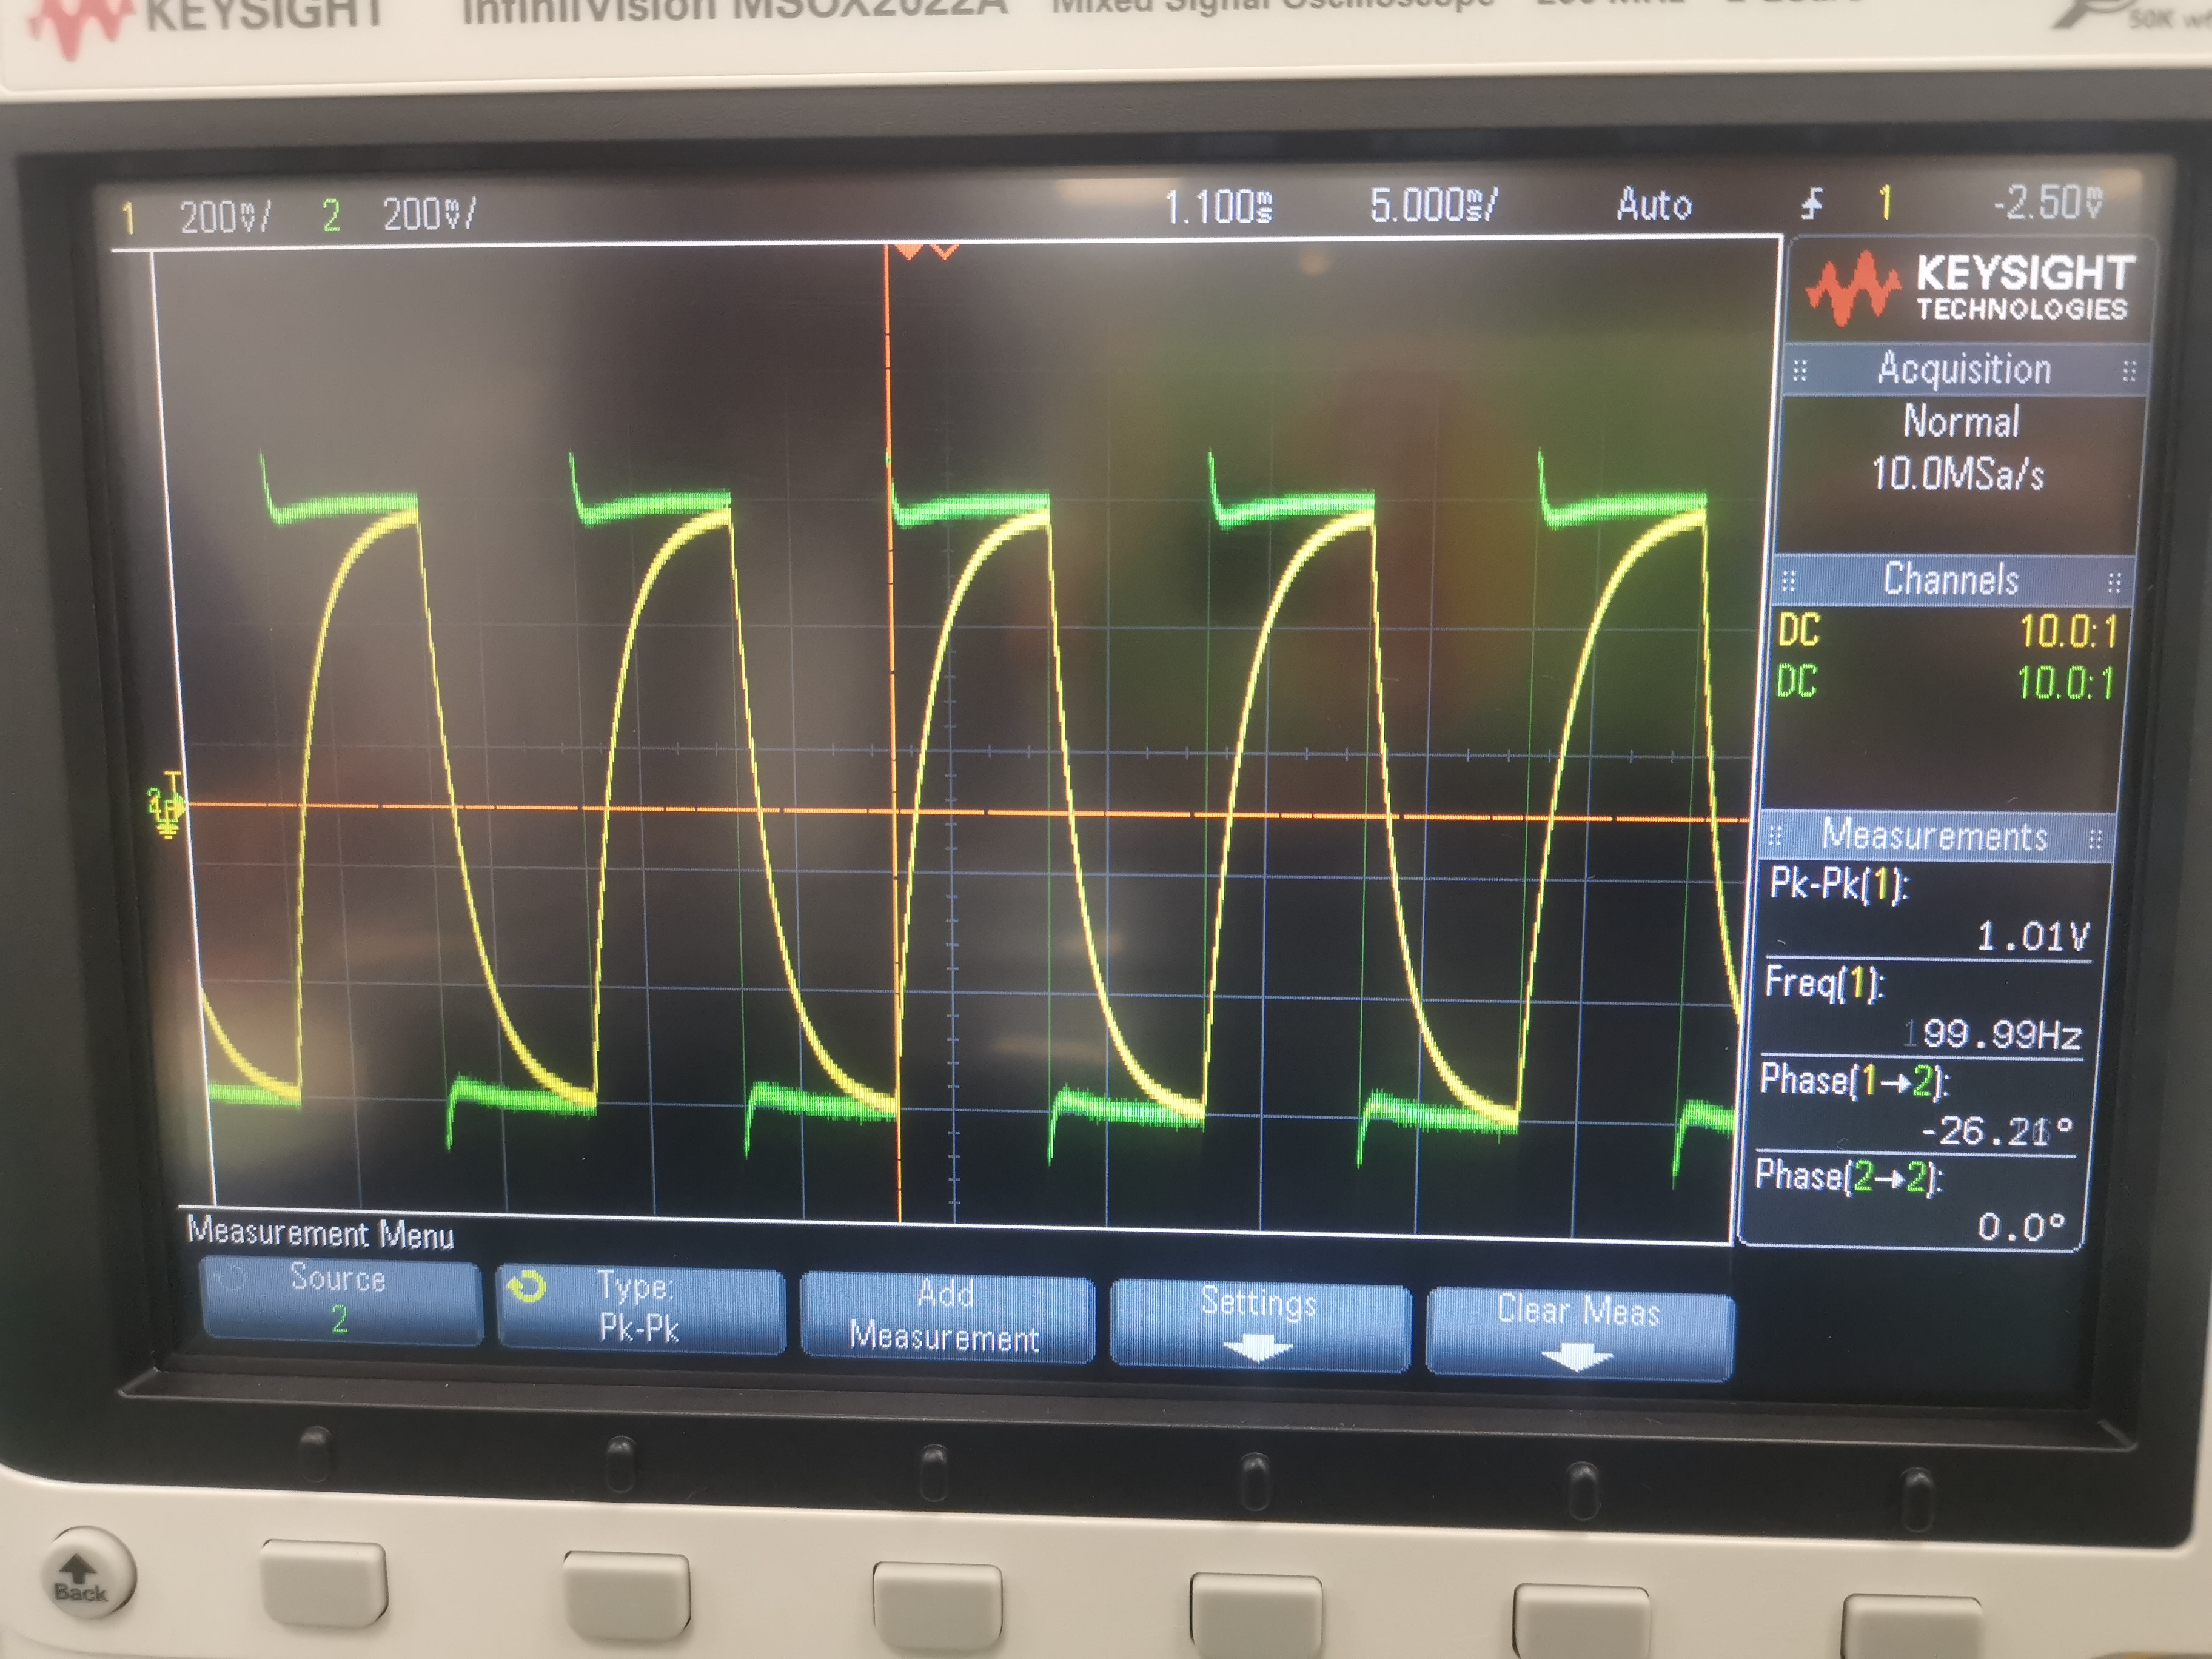
\includegraphics[width=5cm, clip]{step.jpg}
            \caption{Step Response (experimental)}
            \label{step}
        \end{subfigure}
       \begin{subfigure}{0.45\textwidth}
            \begin{tikzpicture}
                \begin{axis} [
                    width=\textwidth,height=0.8\textwidth,
                    xmin=0,
                    xmax=0.005,
                    ymin=0,
                    ymax=1.5,
                    extra x ticks={0},
                    extra y ticks={0},    
                    xlabel style={below right},
                    ylabel style={left},    
                    axis lines=center,
                    xlabel = $V_{out}\ (V)$,
                    ylabel = $t\ (s)$,
                    ]
                    \addplot [
                        domain=0:0.005,
                        samples=30,
                        color=blue,
                    ]
                    {1-exp(-1000*x)};
                    \addlegendentry{$Step Response$}
                \end{axis}
            \end{tikzpicture}
            \caption{Step Response (theoretical)}
            \label{plot:SRb}
        \end{subfigure}
        \caption{Step Response}
        \label{steptrue}
    \end{figure}

    \subsection{Impulse Response}
    The impulse response (Vpp: 100mV, width: 1ms) is shown in \autoref{ima}. The impulse response (Vpp: 200mV, width: 0.5ms) is shown in \autoref{imb}. 
    \begin{figure}[h]
        \centering
        \begin{subfigure}{0.45\textwidth}
            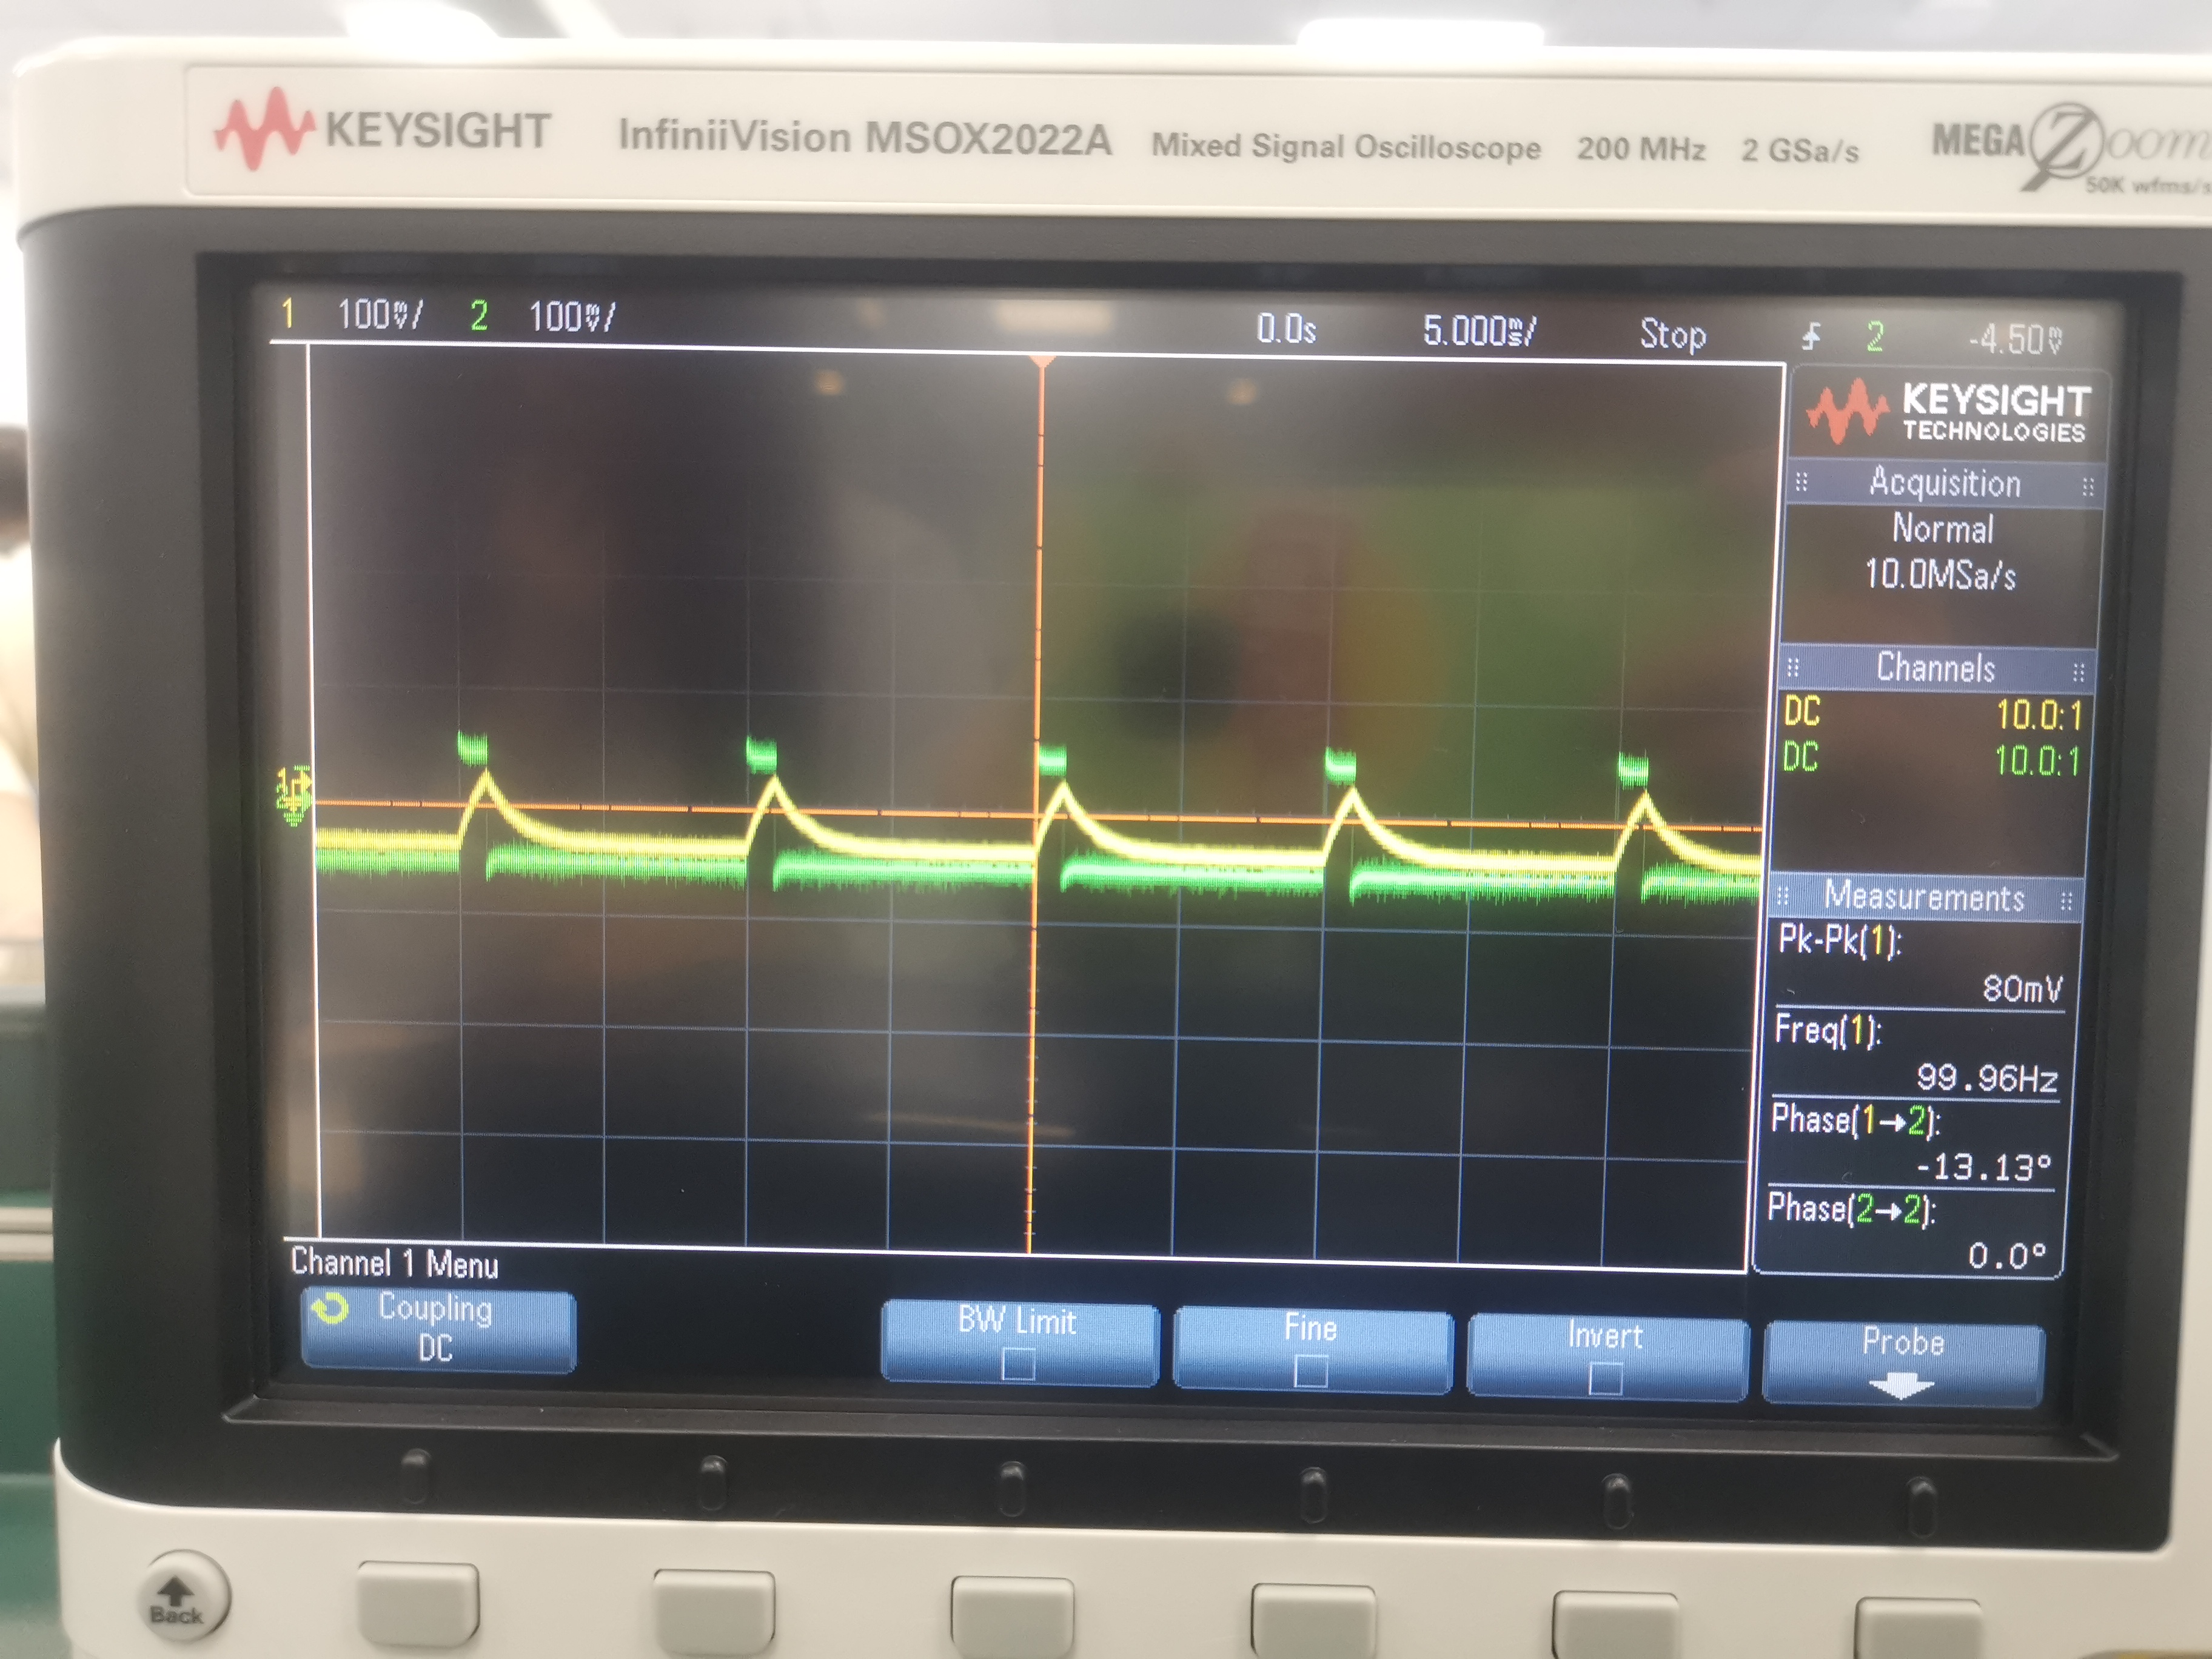
\includegraphics[width=5cm]{impulse1.jpg}
            \caption{Pulse Reponse with Vpp:100mV \& width:1ms}
            \label{ima}
        \end{subfigure}
        \begin{subfigure}{0.45\textwidth}
            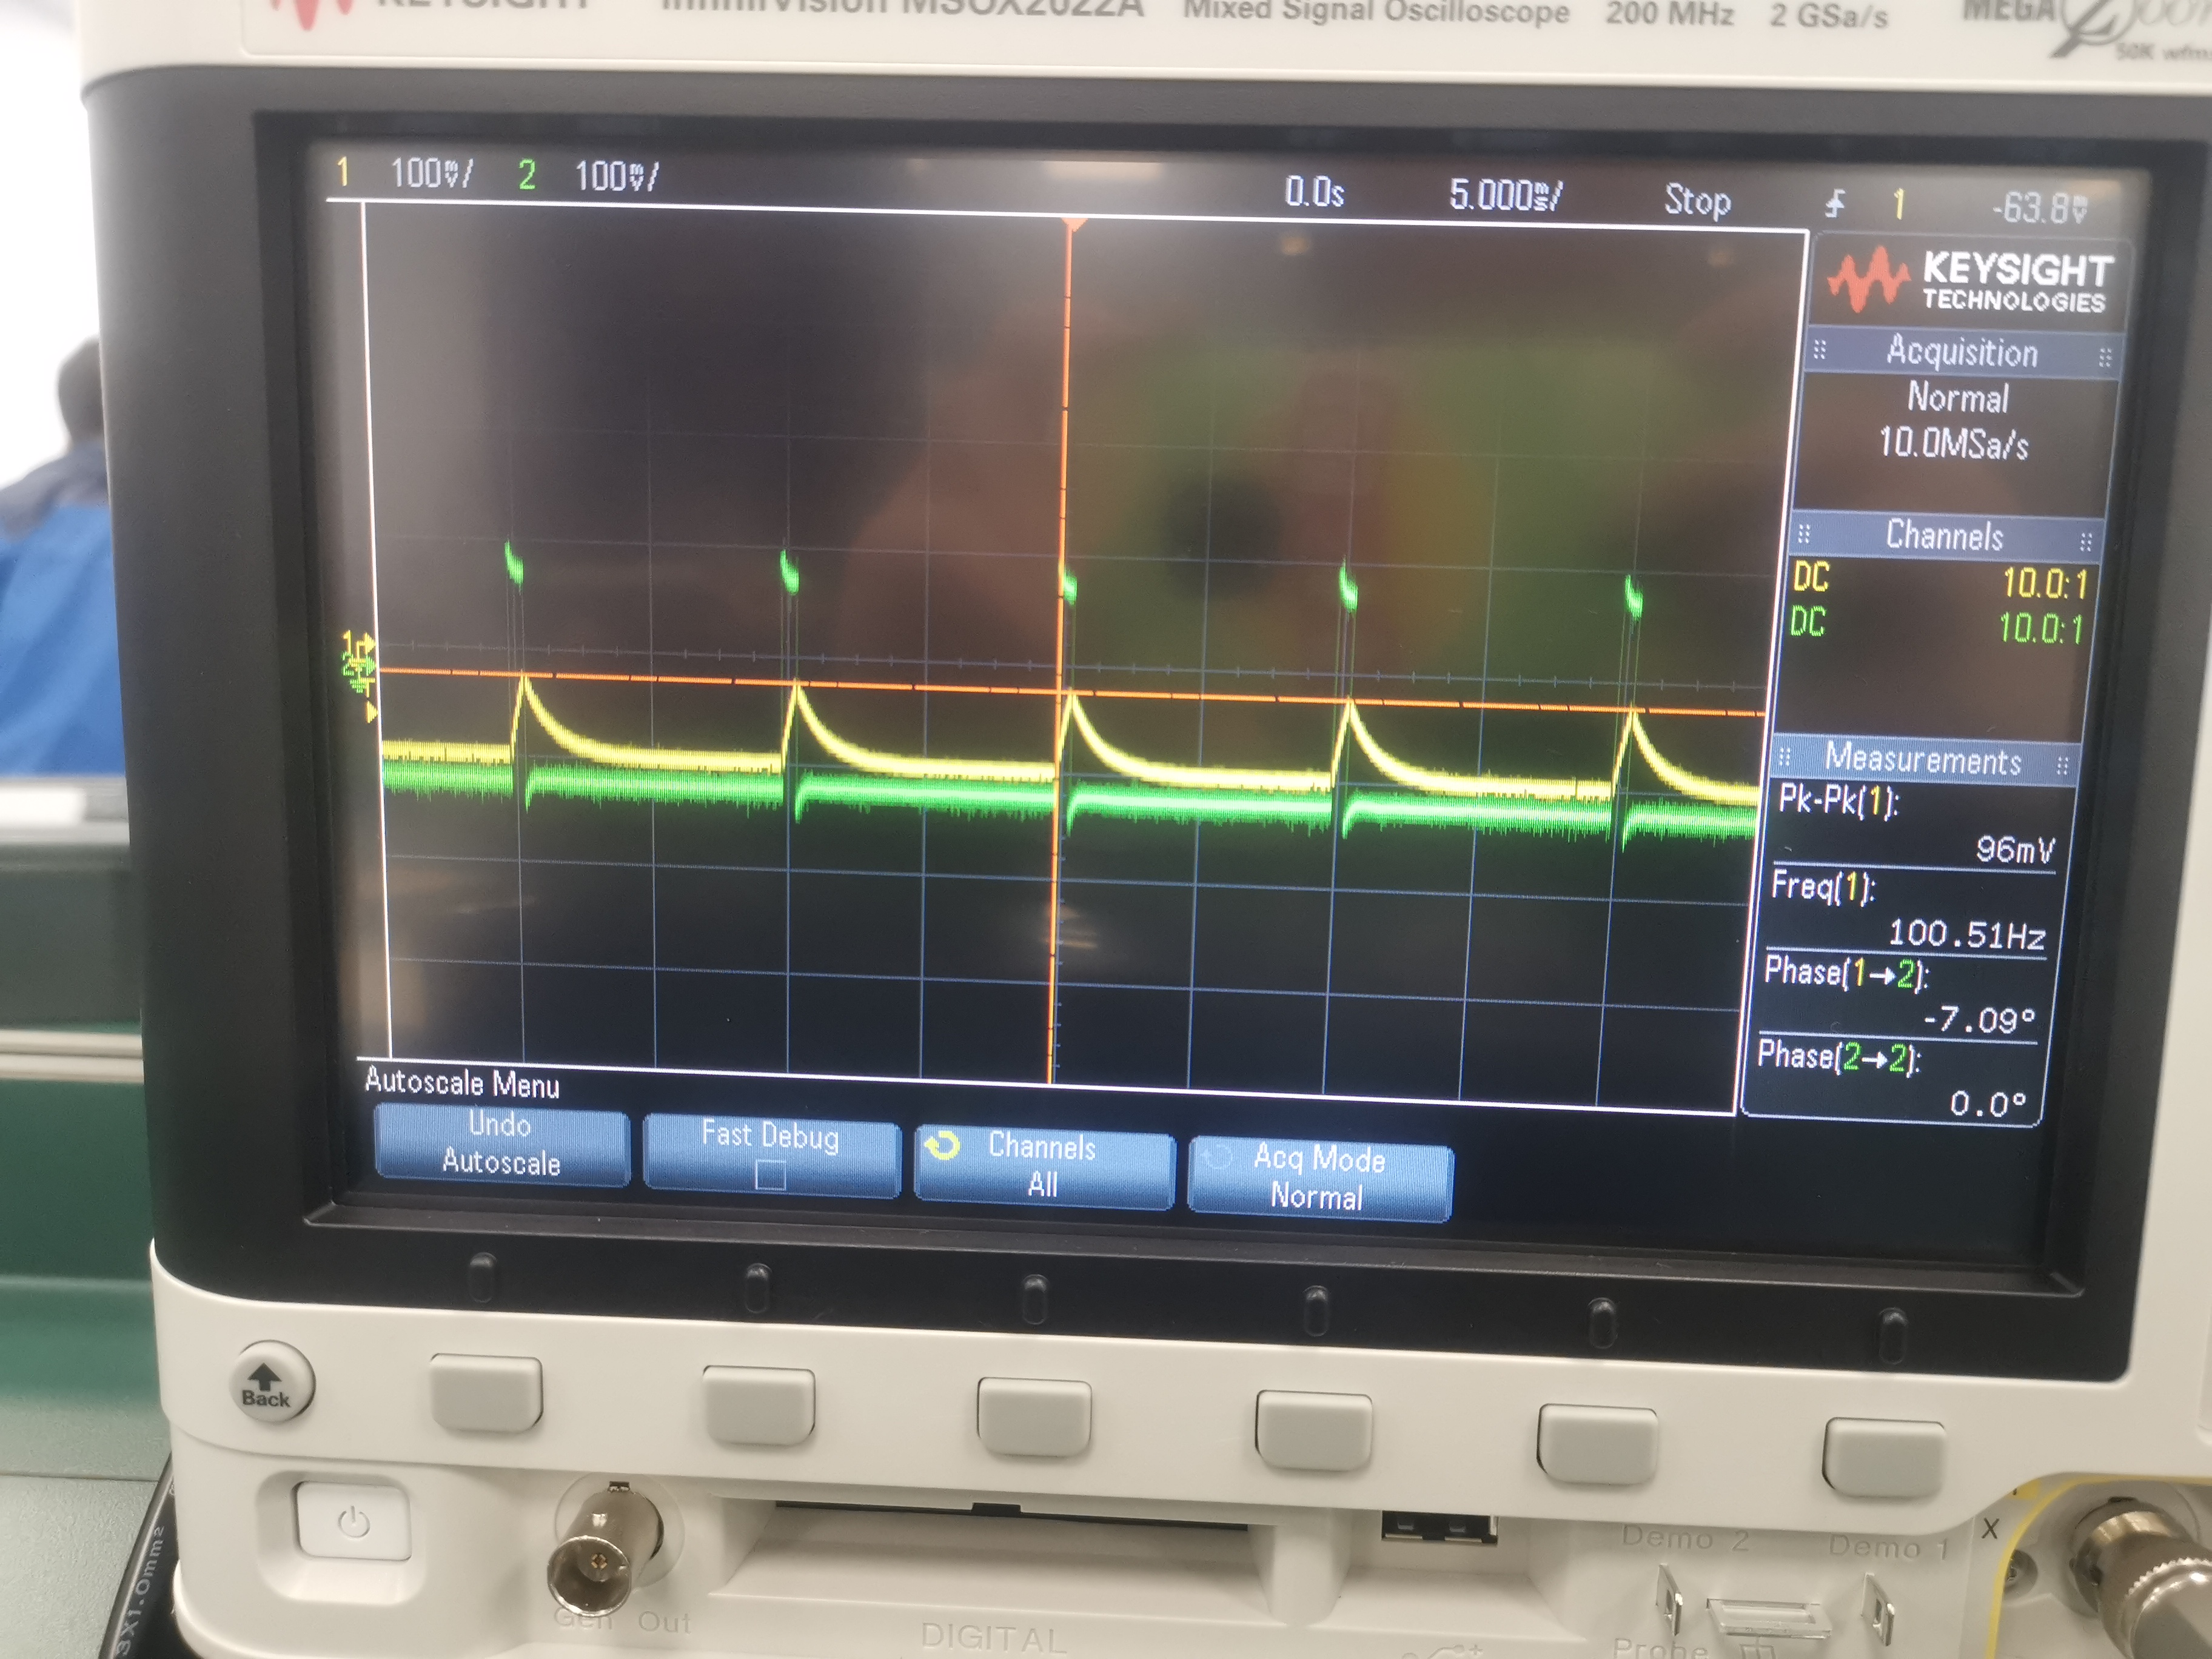
\includegraphics[width=5cm]{impulseb.jpg}
            \caption{Pulse Reponse with Vpp:200mV \& width:0.5ms}
            \label{imb}
        \end{subfigure}
        \caption{Pulse Reponse}
        \label{fig:PR}
    \end{figure}
    We can see that the $V_{out}$ of two impulse response is similar. And smaller width will cause more similarity between the theoretical one and experimental one.
    \begin{equation*}
        h(t) = \frac{e^{-t/RC}}{RC}
    \end{equation*}

    \subsection{Ramp Response}
    The ramp response (Vpp: 100mV \& frequency: 100Hz) is shown in \autoref{ramp}.
    \begin{figure}[h]
        \centering
        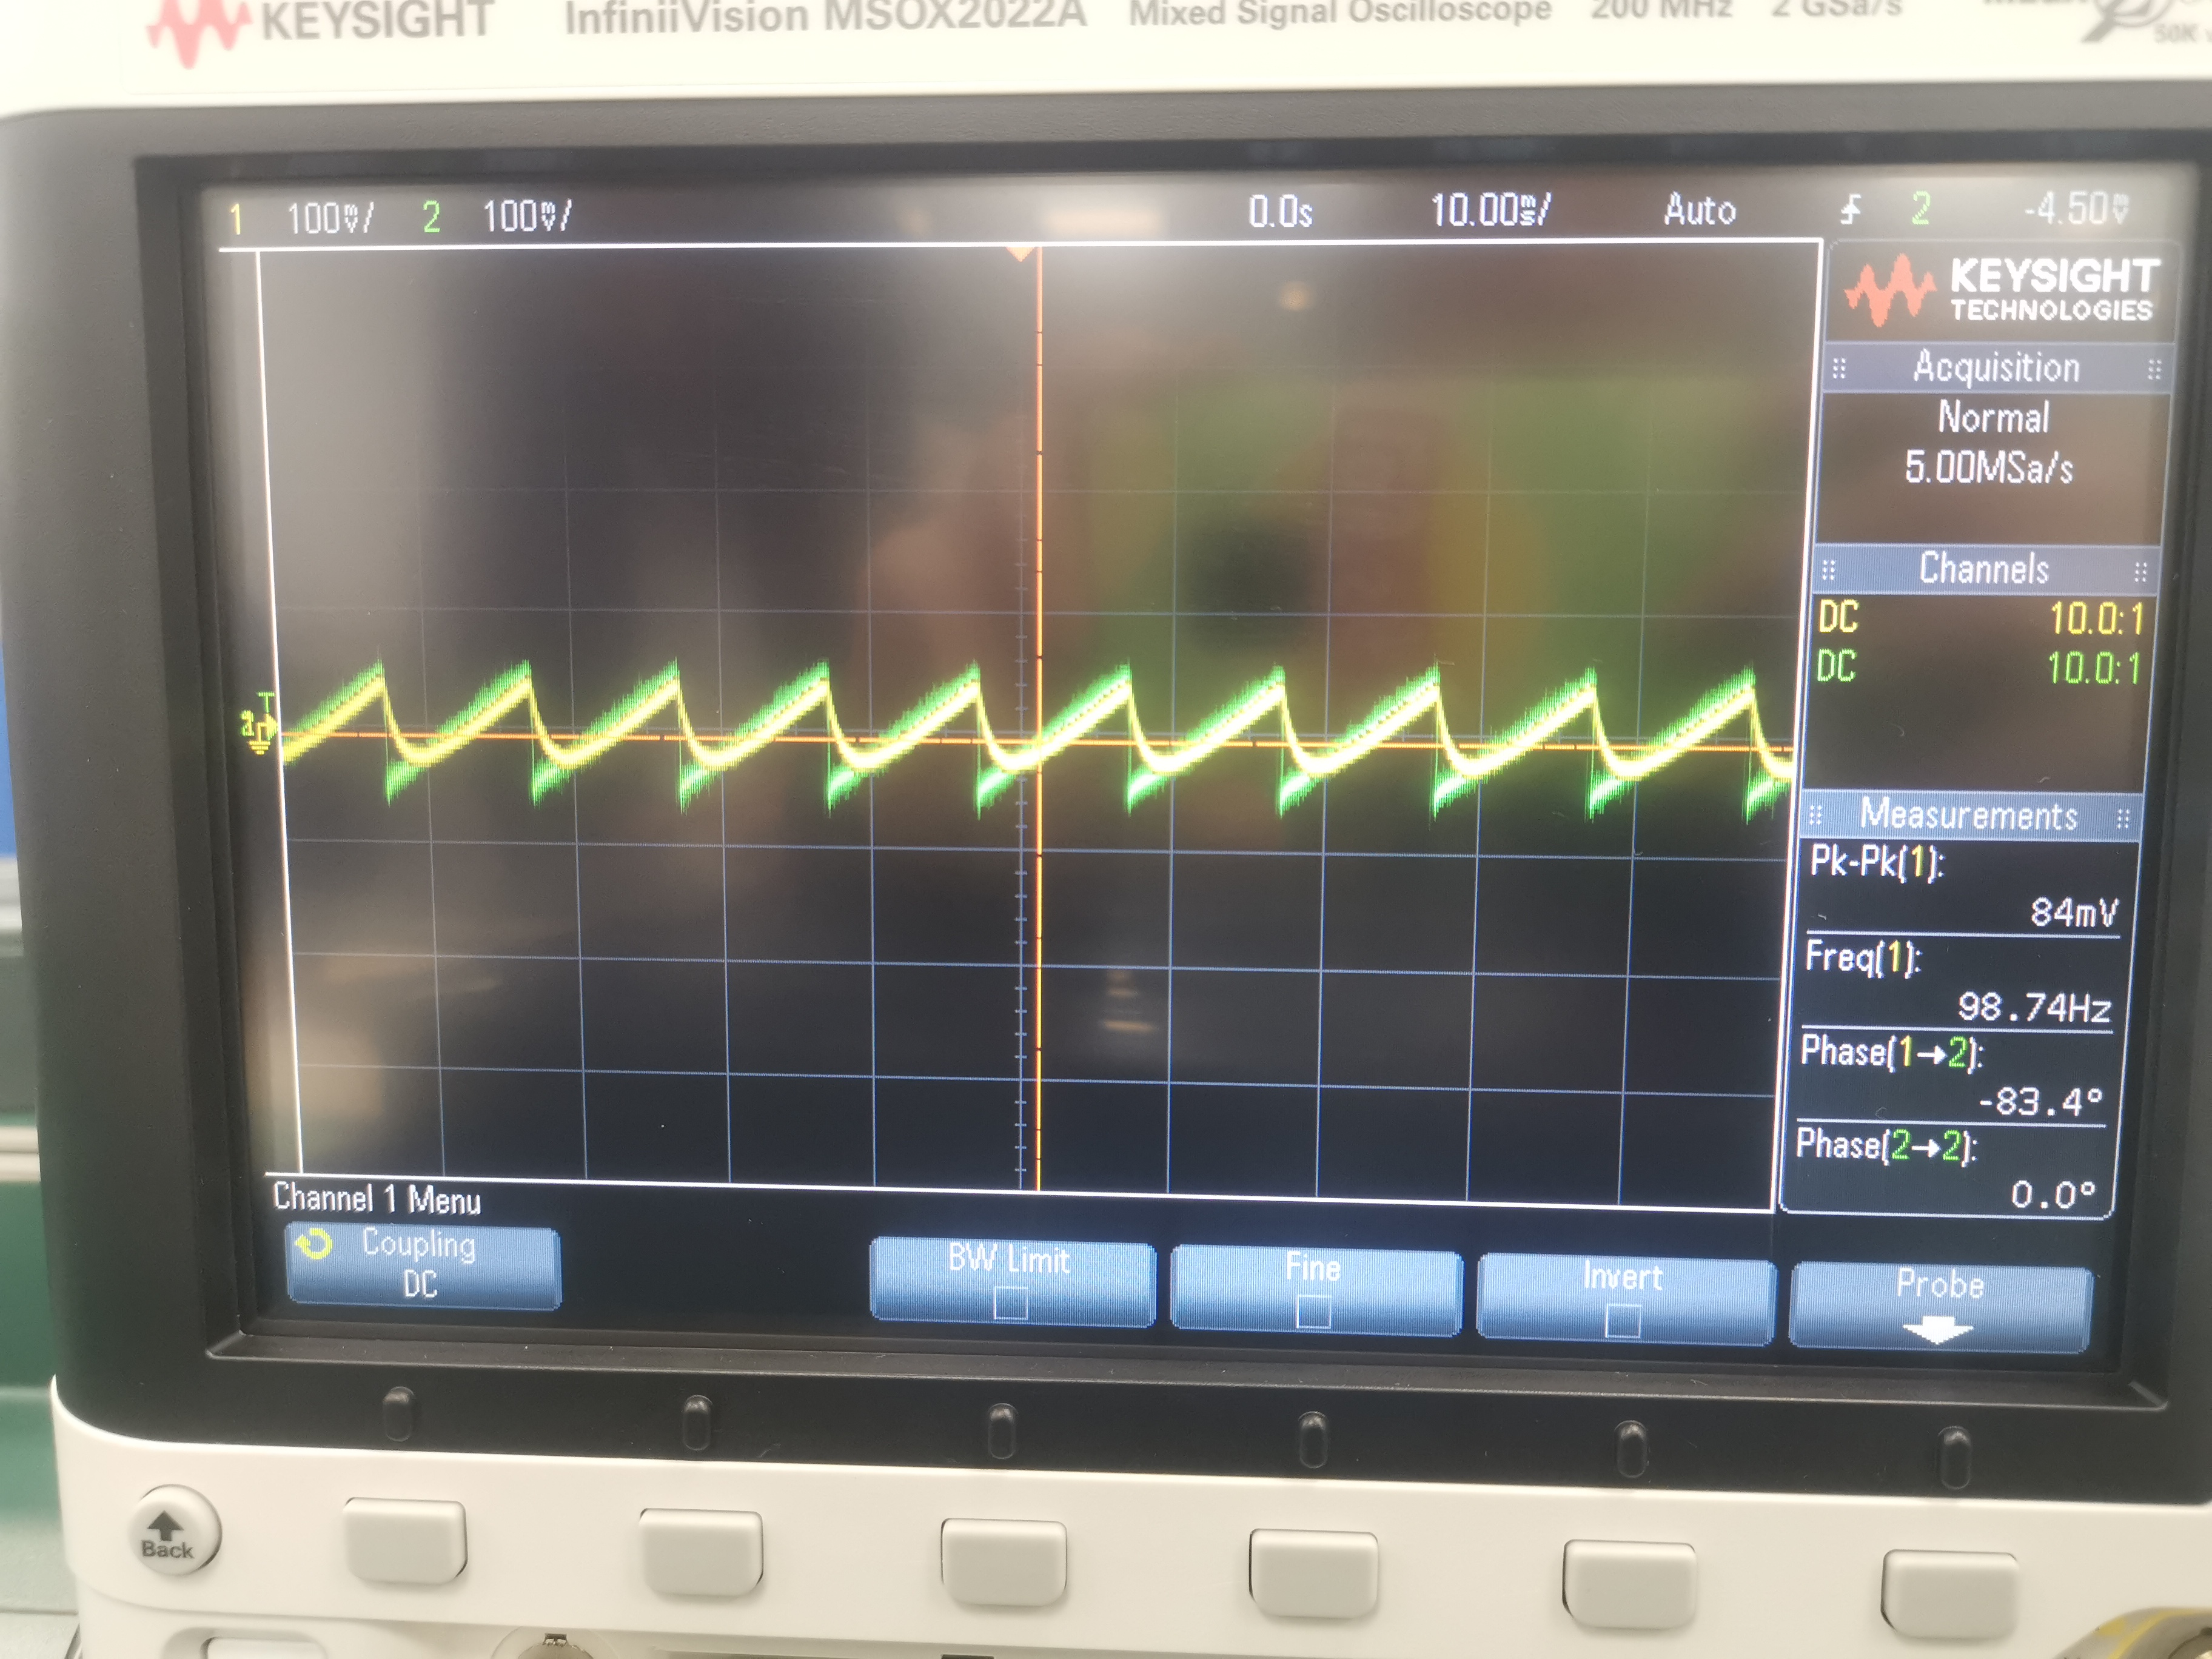
\includegraphics[width=6.5cm]{ramp.jpg}
        \caption{Pulse Reponse with Vpp: 100mV \& frequency: 1000Hz}
        \label{ramp}
    \end{figure}

    \subsection{Sine Reponse}
    The experimental response is shown in \autoref{fig:SR}.
    \begin{figure}[h]
        \centering
        \begin{subfigure}{0.32\textwidth}
            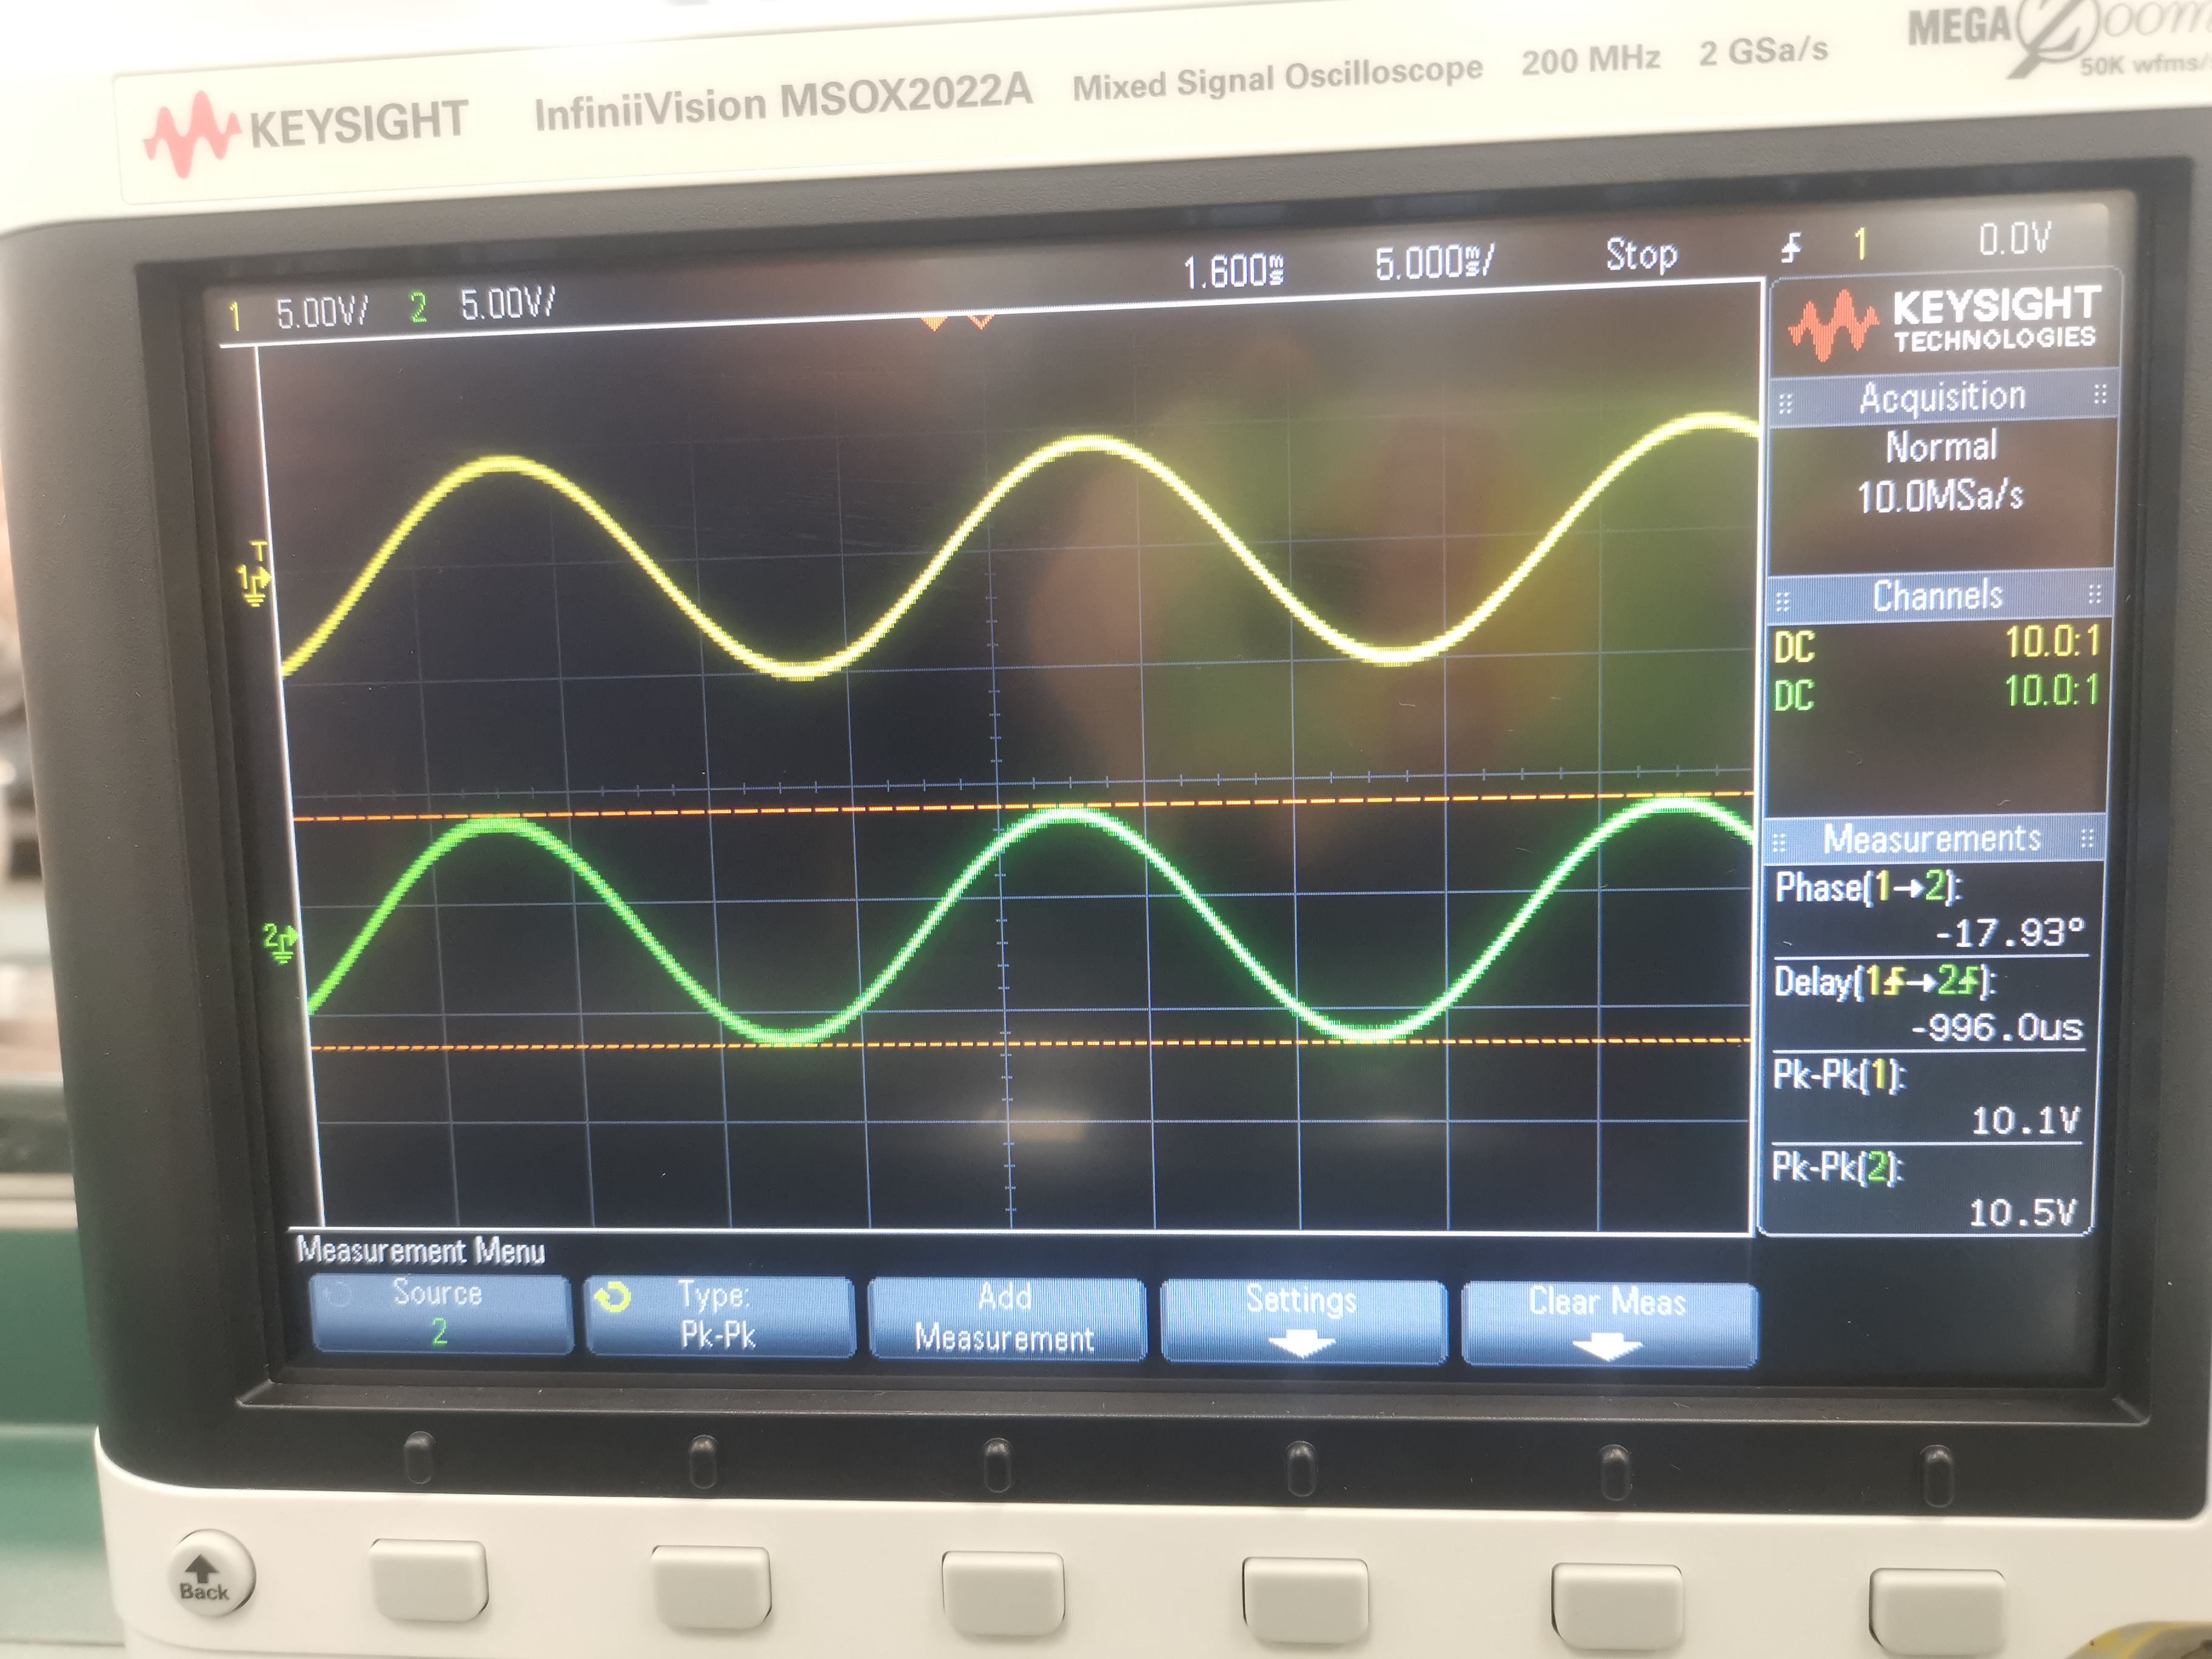
\includegraphics[width=\textwidth, trim={0 1cm 7cm 1cm}, clip]{50.jpg}
            \caption{50Hz}
        \end{subfigure}
        \begin{subfigure}{0.326\textwidth}
            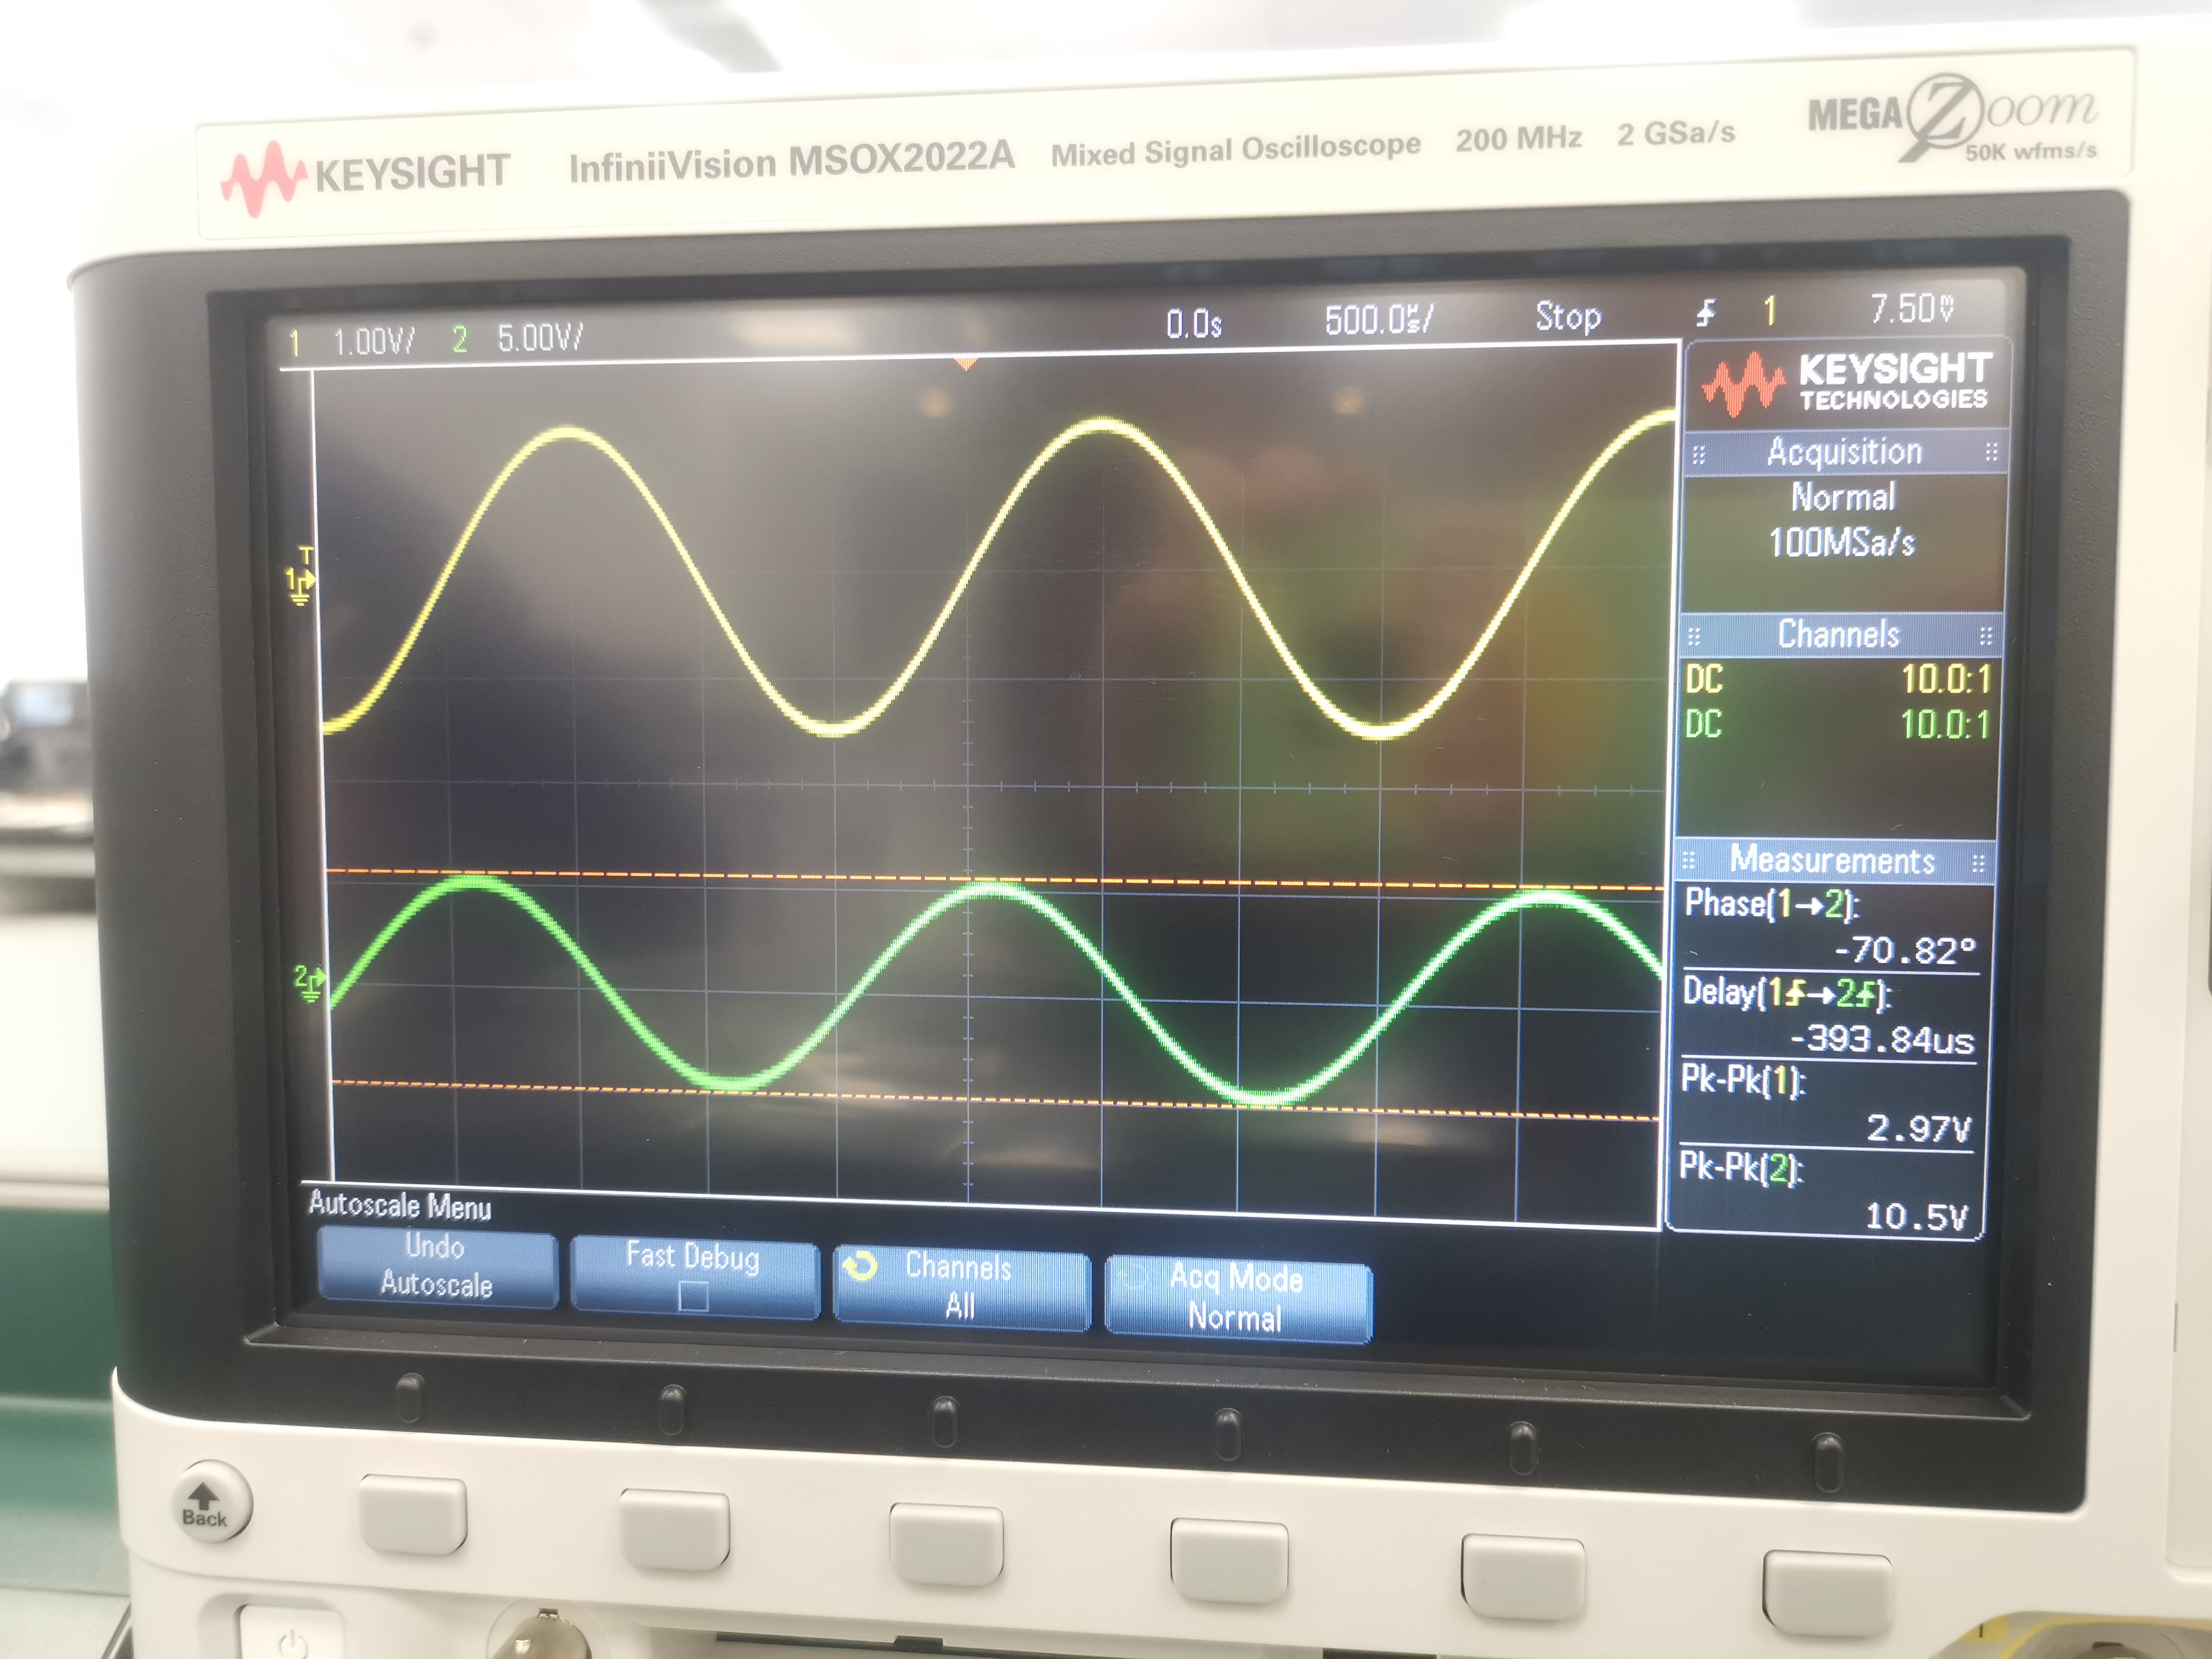
\includegraphics[width=\textwidth, trim={0 1cm 7cm 1cm}, clip]{500.jpg}
            \caption{500Hz}
        \end{subfigure}
        \begin{subfigure}{0.32\textwidth}
            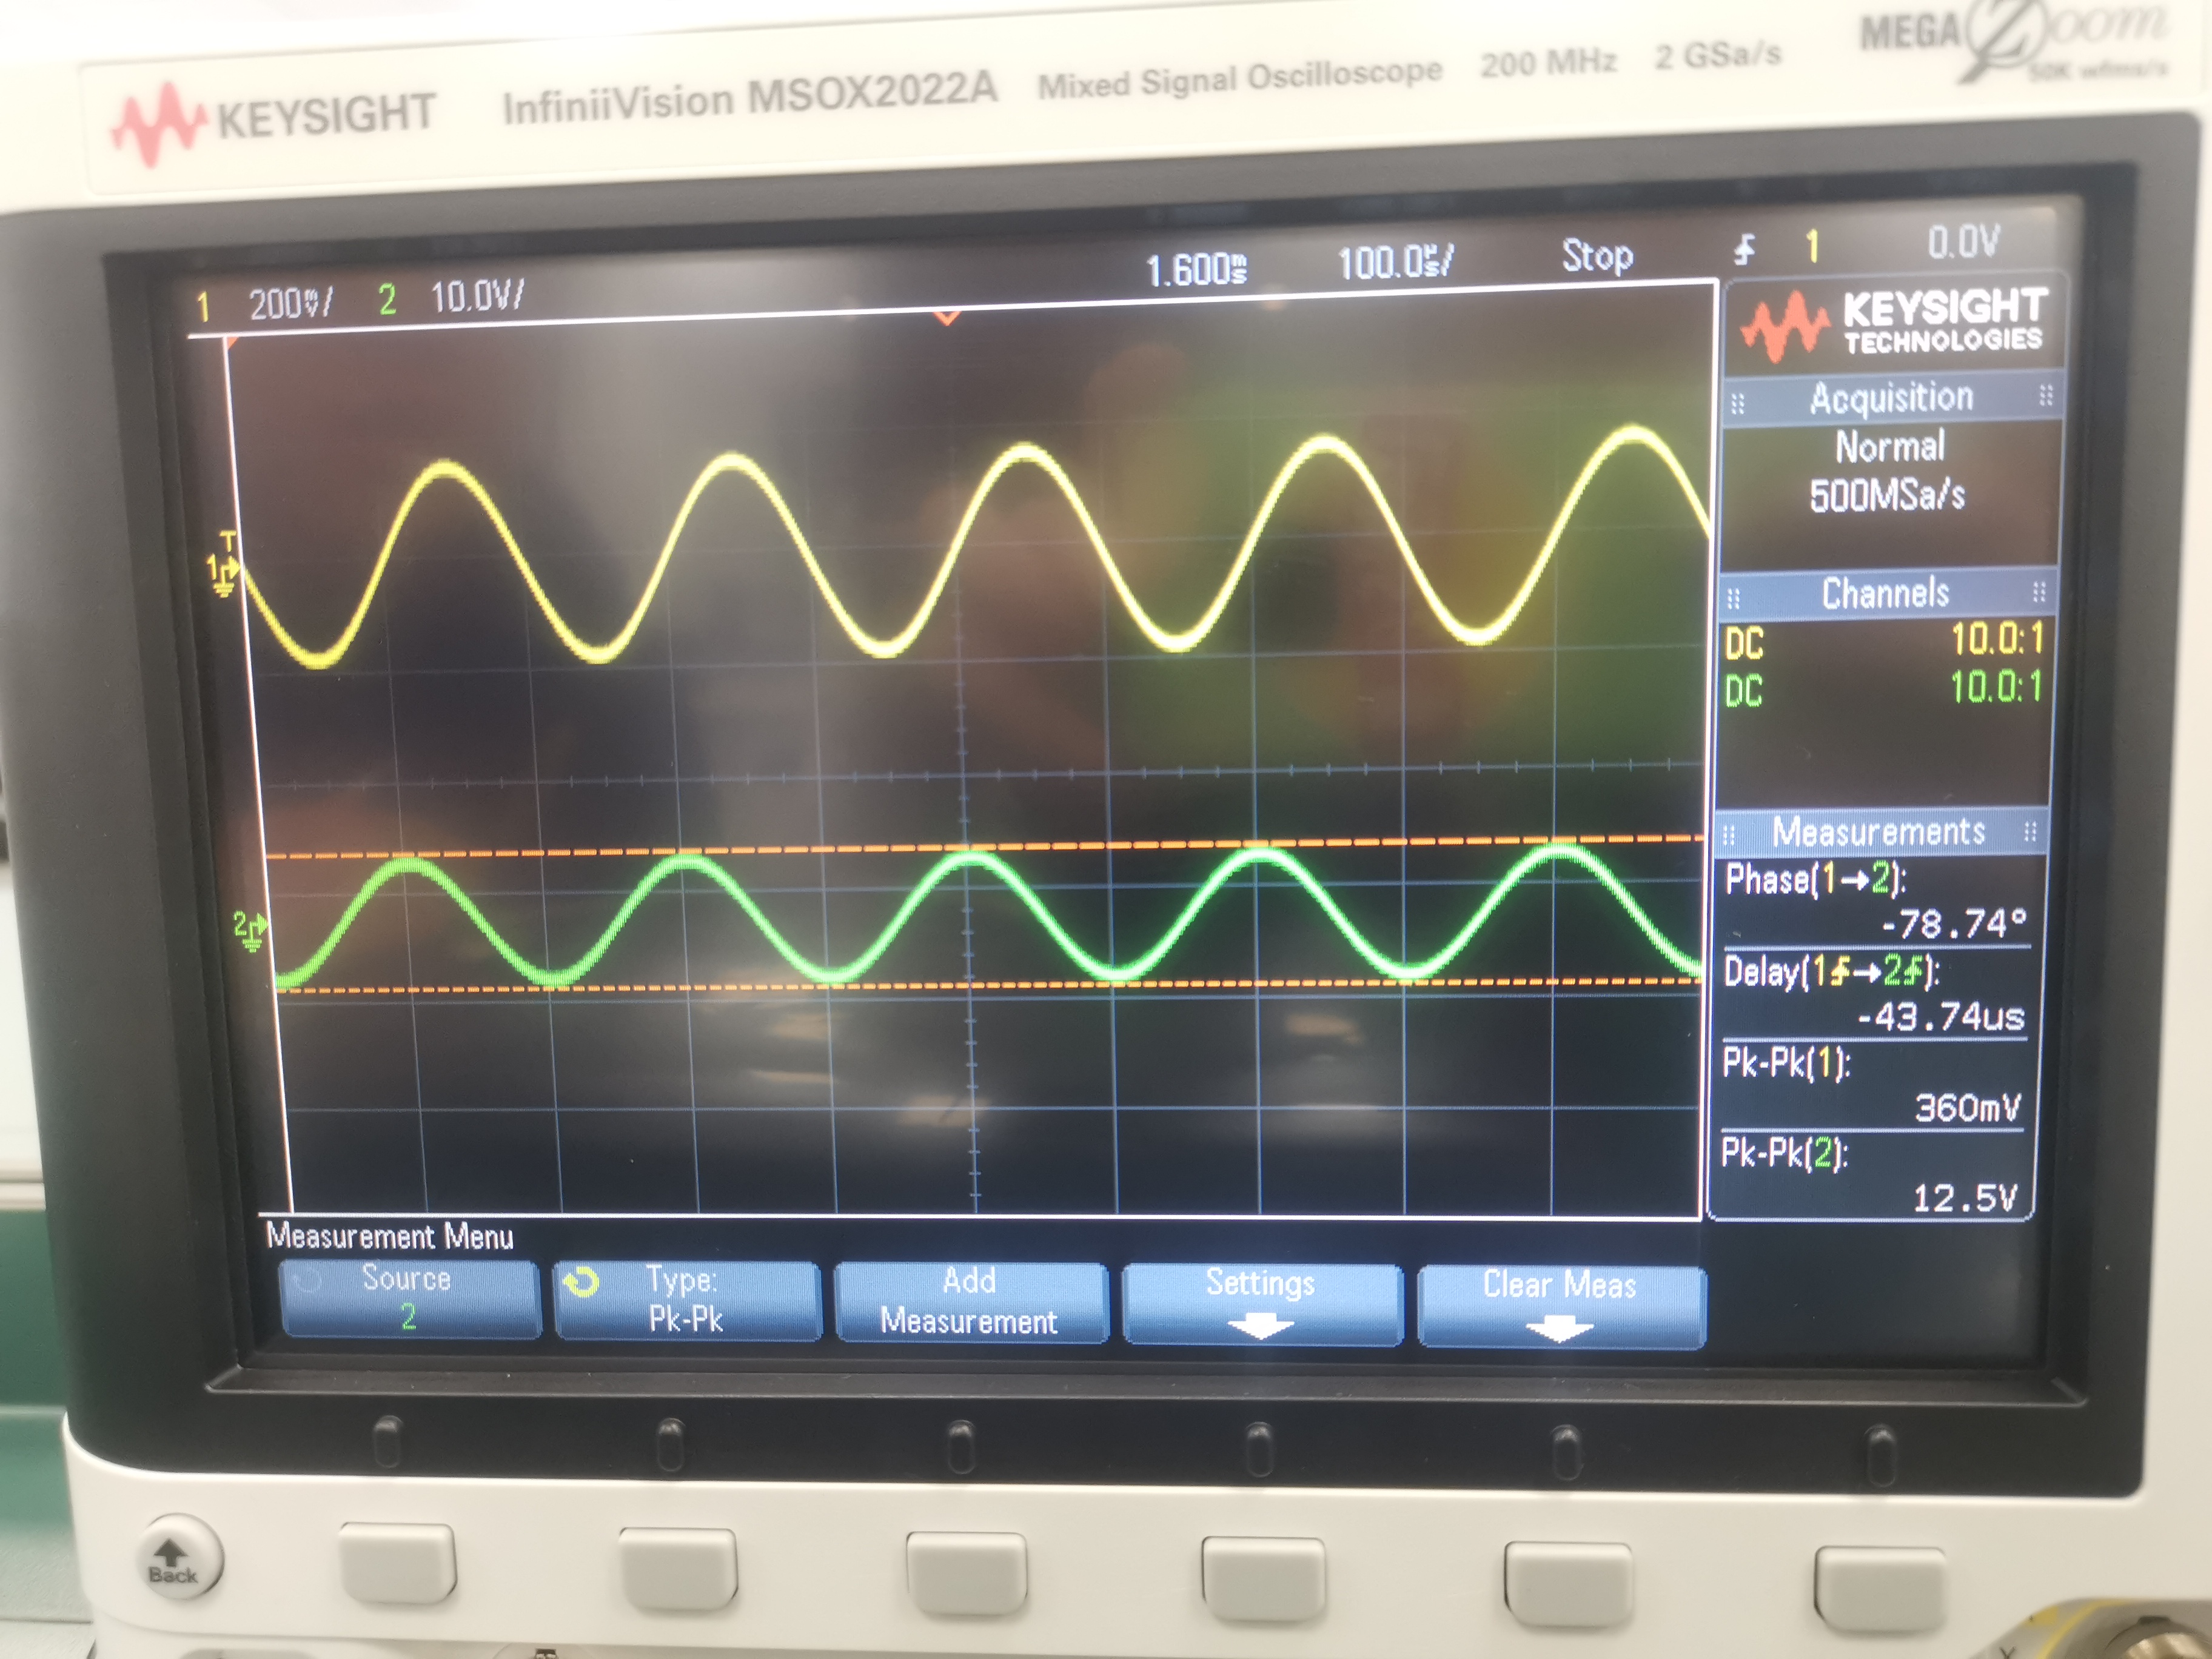
\includegraphics[width=\textwidth, trim={0 1cm 7cm 1cm}, clip]{5000.jpg}
            \caption{5kHz}
        \end{subfigure}
        \caption{Sine Reponse (Vpp: 10V)}
        \label{fig:SR}
    \end{figure}
    Then the compare experimental results iwith the theoretical results calcutaled in prelab in \autoref{tab:SR}.
    \begin{table}[h]
        \centering
        \begin{tabular}{|ccccccccc|}
            \hline
            Freq (Hz) & Vin & Vout & \multicolumn{2}{c}{$|H(j\omega)|$} & \multicolumn{2}{c}{Time Shift}(ms) & \multicolumn{2}{c|}{Phase Shift($^{\circ}$)} \\
              & & & E & T & E & T & E & T \\
            \hline
            50 & 5.05 & 5.25 & 0.962 & 0.954 & 0.996 & 0.967 & -17.93 & -17.44\\
            500 & 1.485 & 5.25 & 0.283 & 0.303 & 0.394 & 0.402 & -70.82 & -72.34\\
            5000 & 0.18 & 6.25 & 0.029 & 0.038 & 0.044 & 0.049 & -78.74 & -88.177\\
            \hline
        \end{tabular}
        \caption{Sine Reponse: \textbf{E}xperimental results v.s. \textbf{T}heoretical results}
        \label{tab:SR}
    \end{table}
    And we can see that the when the frequency is not that big, the theoretical results and experimental results are close to each other.

    \subsection{Discussion \& Error Anlaysis}
   After comparing the simulated results and the theoretical results, we can find that he theoretical results and experimental results are close to each other. However, the magnitude of transfer function $|H(j\omega)|$, phase shift and time shift are all a little bit smaller than expected. It may cause by the cursor position and the system error of oscillator.


    \section{Conclusion}
    In this lab, we analyzed the LTI system (RC circuit)'s reponses with different input signals (step, impulse, square, ramp and sine signal).
    \begin{enumerate}
        \item The impulse response of LTI system can be calculated in two ways.  One is calculate the derivative of step response. And the other is use two step response with small width to simulate it.
        \item For response to sine input, the input with higher frequency will have lower magnitude of the transfer function, smaller time shift and greater phase shift.
    \end{enumerate}

\end{document}